\documentclass[conference]{IEEEtran}
\usepackage{graphicx}
\usepackage{booktabs}
\usepackage{amsmath}
\usepackage{array}
\usepackage{cite}
\usepackage{url}
\usepackage[hidelinks]{hyperref}
\usepackage{flushend}

\begin{document}
\title{Design and Implementation of a Secure Digital Evaluation System\\with Human-Reviewed Marking Analytics}
\author{\IEEEauthorblockN{Shaik Naveed Ahamed}
\IEEEauthorblockA{School of Computer Science and Engineering\\REVA University, Bengaluru, India}}
\maketitle

\begin{abstract}
Paper-based examination evaluation requires physical script handling, manual tabulation and separate records for moderation. This paper presents an implemented Digital Evaluation System (DES) that supports examination setup, private answer-script storage, anonymised assignment, online marking, draft saving, reason-tracked moderation, result publication and student result access. The web application provides role-specific interfaces for Controllers, Evaluators, Moderators and Students, together with an Intelligent Evaluation Analytics dashboard. Access is restricted using database row-level security and server-validated workflow functions; student identity is separated from the script records visible to markers. An independently deployed Python FastAPI service applies scikit-learn Isolation Forest to selected numerical marking features and returns anomaly scores for human review. The analytics path cannot modify examination marks. The implementation is evaluated through source inspection, automated application and service tests, and a live service health check. All 19 application tests and two Python service tests passed, and the deployed service returned the expected healthy response. These results verify the tested implementation behaviour; they do not establish improved marking accuracy, reduced evaluation time or anomaly-detection effectiveness on institutional examinations.
\end{abstract}

\begin{IEEEkeywords}
digital evaluation, on-screen marking, examination workflow, row-level security, audit trail, moderation, anomaly detection, Isolation Forest
\end{IEEEkeywords}

\section{Introduction}
Examination evaluation involves more than displaying a scanned answer script. An operational system must control who can access each script, preserve candidate confidentiality, validate marks, record moderation decisions and release results only after the required workflow is complete. Manual coordination of these activities can fragment records across paper sheets, spreadsheets and messages, making the process difficult to trace.

On-screen marking changes the medium through which examiners access scripts, but its adoption should not itself be treated as evidence of improved assessment quality. Johnson et al.\ compared on-screen and paper marking of extended responses and emphasised empirical evaluation of marking reliability \cite{johnson2010}. Accordingly, the work presented here is an engineering implementation study rather than a claim that digitisation inherently improves marking.

The implemented DES contributes: (i) a role-based workflow from examination setup to published student results; (ii) database-enforced record access, separate student identity mapping and reason-tracked moderation; and (iii) an Isolation Forest analytics service whose output is advisory and linked to a moderator review queue. This paper documents only behaviour present in the implementation and distinguishes functional verification from educational or operational effectiveness.

\begin{figure*}[t]
\centering
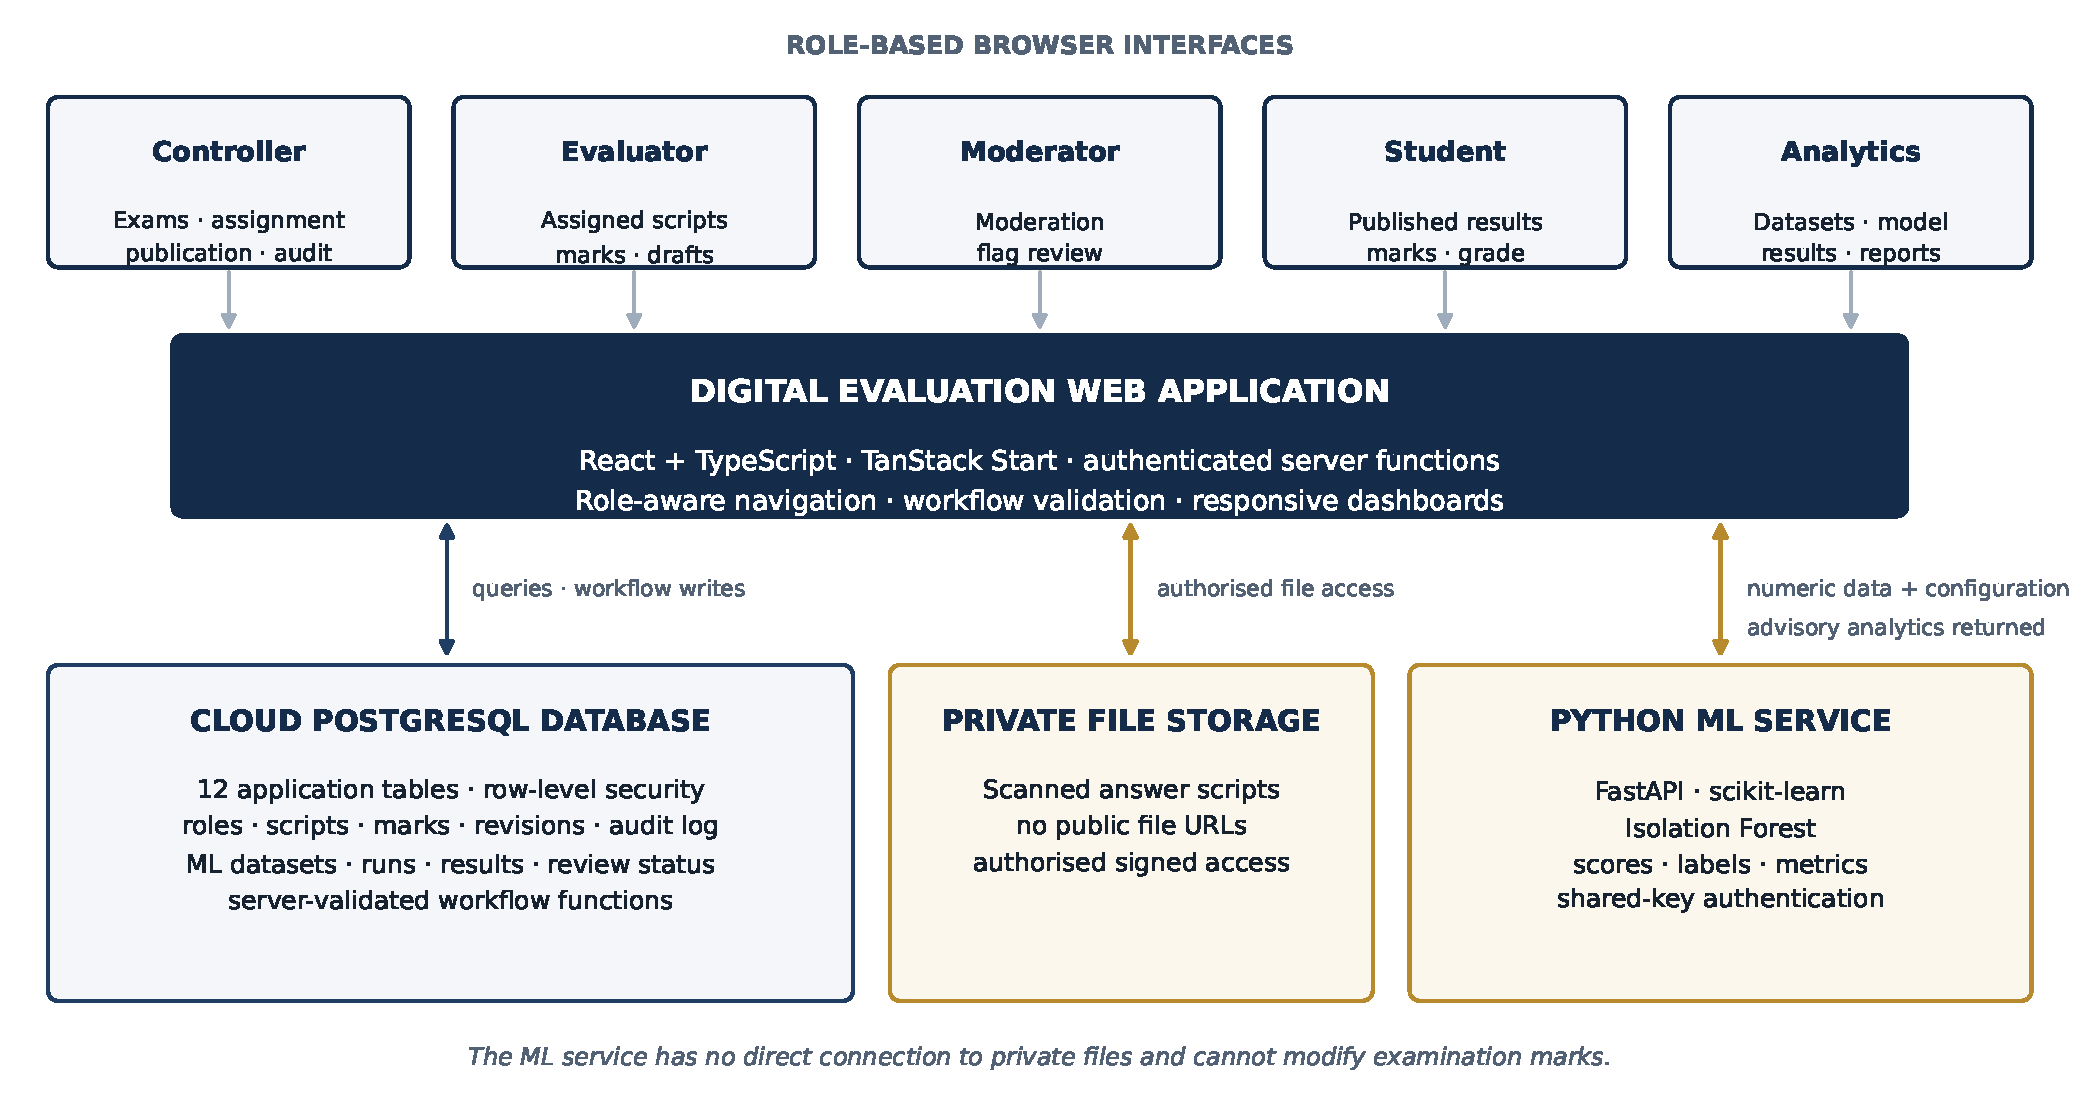
\includegraphics[width=0.98\textwidth]{system-architecture.pdf}
\caption{Implemented DES architecture. The web application mediates access to the cloud database and private script storage. Selected numerical data are sent to the independent Python service, which returns advisory anomaly analytics; the service has no direct path to marks or private files.}
\label{fig:architecture}
\end{figure*}

\section{Methodology}
\subsection{Design and implementation approach}
A design-and-implementation method was used. Requirements were decomposed into four role workflows and one analytics workflow, mapped to a relational data model, and implemented as a responsive React and TypeScript web application using TanStack Start. The backend uses a managed cloud PostgreSQL database, authentication and private file storage. Machine-learning processing is isolated in a Python FastAPI service so that numerical analysis is performed by scikit-learn rather than reproduced in the web client \cite{pedregosa2011}.

Fig.~\ref{fig:architecture} shows the deployed boundaries. The Controller dashboard manages examinations, questions, scripts, assignment, publication, audit records and analytics. Evaluators receive assigned anonymised scripts and enter question-level marks and remarks. Moderators review submitted work and record reasons for changes. Students access their own published results. The analytics dashboard accepts CSV or Excel datasets and snapshots of evaluated scripts, stores run configurations and outputs, and provides filters, history and exports.

\subsection{Evaluation workflow and data model}
The database contains 12 application tables: profiles, user roles, examinations, questions, scripts, script ownership, marks, mark revisions, audit events, ML datasets, ML runs and ML results. Scanned scripts are stored separately in private storage; script rows hold file references. Student identity is held in the script-ownership table rather than in the script record used by markers.

A script progresses through \emph{unassigned}, \emph{assigned}, \emph{evaluated} and \emph{moderated} states. The Controller creates the examination and assigns or reassigns staff within the permitted state transitions. Evaluators may save partial drafts, but final submission requires a value for every question. Moderation is available after evaluation. For question $i$, the result calculation uses
\begin{equation}
f_i = \begin{cases}
m_i, & m_i \text{ is present},\\
e_i, & \text{otherwise},
\end{cases}
\qquad F=\sum_{i=1}^{n}f_i ,
\end{equation}
where $e_i$ is the evaluator mark and $m_i$ is the moderated mark. Publication is rejected while any script in the examination remains unmoderated. The current result view uses fixed bands O ($\geq90\%$), A+ ($\geq80\%$), A ($\geq70\%$), B+ ($\geq60\%$), B ($\geq50\%$), C ($\geq40\%$) and F below $40\%$; these are prototype settings, not a claim about institutional regulations.

\subsection{Access control and audit design}
Role membership is stored in a protected role table and checked by a database function. Row-level security (RLS) restricts rows returned or changed through normal database access \cite{postgresqlRLS}. Evaluator and moderator visibility is based on assignment, while student access requires script ownership and a published examination. Controllers administer records and review audit events. Examinations and questions use the same access predicate as their scripts.

Assignment, reassignment, draft saving, evaluation submission, moderation and publication are implemented as server-validated database functions. They check role or assignment, workflow state and question limits. A changed moderated mark requires a non-empty reason; the old value, new value, reason, actor and timestamp are inserted into the mark-revision table in the same database transaction. Private file policies permit Controller management and assigned-staff reading. These controls reduce unauthorised access paths, but this paper does not claim that they guarantee complete system security.

\subsection{Human-reviewed anomaly analytics}
The analytics workflow sends user-selected numerical columns to the Python service over HTTPS with a shared-key header. The service accepts 10--20{,}000 records, converts selected values to numeric form, median-imputes missing entries and standardises the feature matrix. Isolation Forest is then fitted with a configurable number of estimators (10--1000), contamination greater than zero and at most 0.5, and a fixed random state of 42 \cite{liu2008}. The negated anomaly score is returned so that larger values indicate more unusual records.

For live snapshots, available features include evaluator and final percentages, moderation difference, question-level mean, spread, minimum and maximum percentages, and the number of written remarks. Uploaded datasets may supply other numerical features. The service reports score summaries, threshold, missing-value count and, where computable, silhouette and group-difference diagnostics. Precision, recall, F1 and a confusion matrix are calculated only when a usable label column is explicitly supplied; labels are not inferred.

Returned scores and classifications are stored as ML results. Moderators can inspect flagged rows, add comments and set \emph{reviewed} or \emph{investigate} status. The review function updates only the analytics result and audit log. No ML code path calls a marking or moderation function, so a prediction cannot change an examination mark.

\subsection{Verification method}
Verification used three evidence sources. First, workflow, schema and policy source files were inspected against the claims in this paper. Second, existing automated tests were rerun: five application test files covering grading, final-mark selection, analytics helpers, dataset profiling, mark bounds and route rendering, plus two FastAPI tests covering authentication rejection and a known-outlier fixture. Third, the deployed service's public health endpoint was queried. No timing experiment, marker-agreement study, penetration test or institutional labelled-dataset evaluation was performed.

\section{Results}
Table~\ref{tab:results} reports the observed verification outcomes. The application run passed 19 tests across five files. Both Python tests passed: a request without the service key was rejected, and the synthetic unit fixture exercised real Isolation Forest fitting, outlier labels and labelled-metric generation. The fixture is a software test, not evidence of accuracy on examination data. A live request to \texttt{/health} returned \texttt{status=ok} and identified \texttt{sklearn.ensemble.IsolationForest}.

\begin{table}[t]
\centering
\caption{Observed implementation verification results}
\label{tab:results}
\begin{tabular}{p{2.25cm}p{4.95cm}}
\toprule
Evidence source & Observed result \\
\midrule
Application tests & 19/19 passed in five test files \\
Python service tests & 2/2 passed; missing-key request rejected and real model path exercised \\
Live ML smoke check & Healthy response received from the deployed FastAPI service \\
Schema inspection & 12 application tables; RLS enabled across the workflow and analytics tables \\
Workflow inspection & Role/state checks, mark bounds, mandatory moderation reasons and publication gate present \\
ML-to-marks boundary & No analytics path writes evaluator marks, moderated marks or totals \\
\bottomrule
\end{tabular}
\end{table}

The implementation therefore satisfies the tested functional invariants: question marks are bounded, moderated values take precedence in final tabulation, moderation changes require reasons, unmoderated examinations cannot be published, and anomaly flags remain advisory. The architecture also separates identity mapping, private files and external numerical processing.

These are limited engineering results. They do not quantify evaluation-time savings, marking accuracy, inter-rater reliability, detection precision on real institutional records or resistance to a dedicated security attack. The fixed grade bands require institutional confirmation. Isolation Forest flags statistical outliers, which may be legitimate records, and uploaded labels may be unsuitable for validation. Consequently, human moderation and a future controlled institutional evaluation remain necessary.

\balance
\section{Conclusion}
The implemented DES integrates private script handling, anonymised role-based assignment, online marking, reason-tracked moderation, automated tabulation and published student results in one workflow. Database policies and validated workflow functions enforce the implemented access and state rules, while revision and audit records preserve evidence of changes. A separate FastAPI and scikit-learn service adds Isolation Forest analytics without granting the model authority to alter marks. Automated tests and the live health check confirm the reported implementation behaviour, but broader claims about efficiency, assessment quality and real-world anomaly accuracy require separate empirical studies.

\begin{thebibliography}{10}
\bibitem{johnson2010}
M.~Johnson, R.~N\'adas, and J.~F.~Bell, ``Marking essays on screen: An investigation into the reliability of marking extended subjective texts,'' \emph{British Journal of Educational Technology}, vol.~41, no.~5, pp.~814--826, 2010. [Online]. Available: \url{https://doi.org/10.1111/j.1467-8535.2009.00979.x}

\bibitem{postgresqlRLS}
The PostgreSQL Global Development Group, ``Row security policies,'' \emph{PostgreSQL Documentation}. [Online]. Available: \url{https://www.postgresql.org/docs/current/ddl-rowsecurity.html}. [Accessed: Nov.~11, 2026].

\bibitem{pedregosa2011}
F.~Pedregosa \emph{et al.}, ``Scikit-learn: Machine learning in Python,'' \emph{Journal of Machine Learning Research}, vol.~12, pp.~2825--2830, 2011. [Online]. Available: \url{https://jmlr.org/papers/v12/pedregosa11a.html}

\bibitem{liu2008}
F.~T.~Liu, K.~M.~Ting, and Z.-H.~Zhou, ``Isolation Forest,'' in \emph{Proc. 8th IEEE Int. Conf. Data Mining (ICDM)}, 2008, pp.~413--422. [Online]. Available: \url{https://doi.org/10.1109/ICDM.2008.17}
\end{thebibliography}
\end{document}
